\chapter{Applications}
\label{ch:Applications}
\section{Introduction}
To measure the performance AUC values will be used. Using AUC values to measure the performance of SDMs has been criticized \parencite{lobo_auc:_2008, jimenez-valverde_insights_2012}. However, most of the issues that are usually raised are not of particular interest in our case. Furthermore, as far as we know there is no other popular and threshold independent performance measure. \\

Before fitting the models he data-sets were splitted into a training and a test set. The training data consists of \nicefrac{3}{4}'th of the data while the test set contains the other \nicefrac{1}{4}'th.\\

\section{Results}
\subsection{Presence-only data}

\begin{table}[!htb]
\center
\begin{tabular}{lcccc}

 & \multicolumn{2}{c}{All variables} & \multicolumn{2}{c}{Bioclimatic variables}\\
\cline{2-3} \cline{4-5} \\
Method & Mean AUC & SE & Mean AUC & SE \\
\midrule
Logistic: vanilla               & 0.933 & 0.036 & 0.889& 0.080 \\
Logistic: backward              & 0.817 & 0.238 & 0.926& 0.031 \\
Logistic: forward               & 0.682 & 0.231 & 0.493& 0.211 \\
Logistic: PCA                   & 0.875 & 0.074 & 0.857& 0.094 \\
Logistic: presence PCA          & 0.779 & 0.205 & 0.855& 0.100 \\
Logistic: background PCA        & 0.877 & 0.077 & 0.872& 0.076 \\
Logistic: kernel PCA            & 0.937 & 0.030 & 0.916& 0.049 \\
Logistic: presence kernel PCA   & 0.946 & 0.031 & 0.924& 0.046 \\
Logistic: background kernel PCA & 0.941 & 0.027 & 0.929& 0.030 \\
Logistic: lasso                 & 0.939 & 0.031 & 0.924& 0.044 \\
Logistic: ridge                 & 0.934 & 0.033 & 0.905& 0.051 \\
Logistic: select07              & 0.931 & 0.039 & 0.900& 0.061 \\
GAM: auto selection             & 0.927 & 0.072 & 0.927& 0.027 \\
GAM: vanilla                    & 0.908 & 0.084 & 0.926& 0.037 \\
GAM: select07                   & 0.936 & 0.046 & 0.929& 0.032 \\
MaxEnt                          & 0.902 & 0.063 & 0.912& 0.042 \\
MaxEnt Vanilla                  & 0.867 & 0.117 & 0.910& 0.044 \\
ANN                             & 0.951 & 0.032 & 0.941& 0.033 \\
ANN: vanilla                    & 0.931 & 0.039 & 0.921& 0.039 \\
GBM                             & 0.958 & 0.030 & 0.941& 0.028 \\
\bottomrule
\end{tabular}
\end{table}


\begin{figure}[!htb]
\center
\makebox[\textwidth][c]{%
	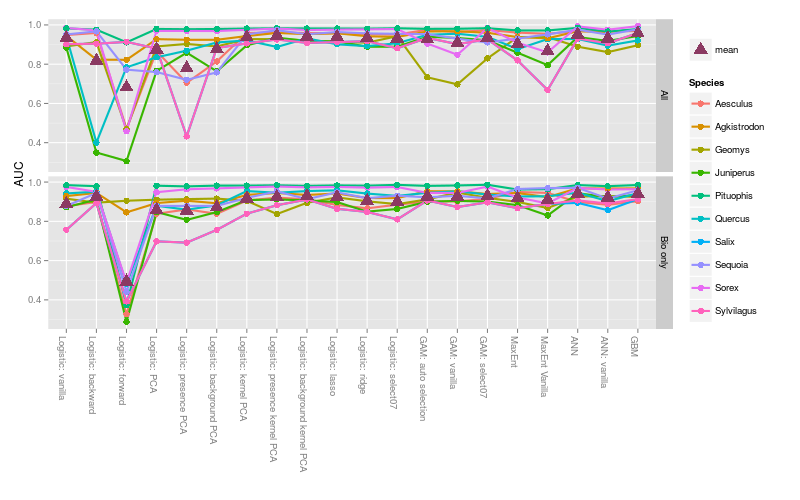
\includegraphics[scale=0.70]{Plots/AUCPlot.png}
}
\end{figure}


\subsection{Presence-absence data}

\begin{table}[!htb]
\center
\begin{tabular}{lcccc}
 & \multicolumn{2}{c}{All variables} & \multicolumn{2}{c}{Bioclimatic variables}\\
\cline{2-3} \cline{4-5} \\
Method & Mean AUC & SE & Mean AUC & SE \\
Logistic: vanilla    & 0.961 & 0.027 & 0.961& 0.027 \\
Logistic: backward   & 0.682 & 0.301 & 0.682& 0.301 \\
Logistic: forward    & 0.774 & 0.284 & 0.774& 0.284 \\
Logistic: PCA        & 0.913 & 0.084 & 0.913& 0.084 \\
Logistic: kernel PCA & 0.950 & 0.052 & 0.950& 0.052 \\
Logistic: lasso      & 0.960 & 0.042 & 0.960& 0.042 \\
Logistic: ridge      & 0.957 & 0.044 & 0.957& 0.044 \\
Logistic: select07   & 0.756 & 0.239 & 0.756& 0.239 \\
GAM: auto selection  & 0.925 & 0.098 & 0.925& 0.098 \\
GAM: vanilla         & 0.877 & 0.117 & 0.877& 0.117 \\
GAM: select07        & 0.948 & 0.062 & 0.948& 0.062 \\
ANN                  & 0.973 & 0.020 & 0.973& 0.020 \\
ANN: vanilla         & 0.962 & 0.036 & 0.962& 0.036 \\
GBM                  & 0.977 & 0.014 & 0.977& 0.014 \\
\bottomrule

\end{tabular}
\end{table}




\begin{figure}[!htb]
\center
\makebox[\textwidth][c]{%
	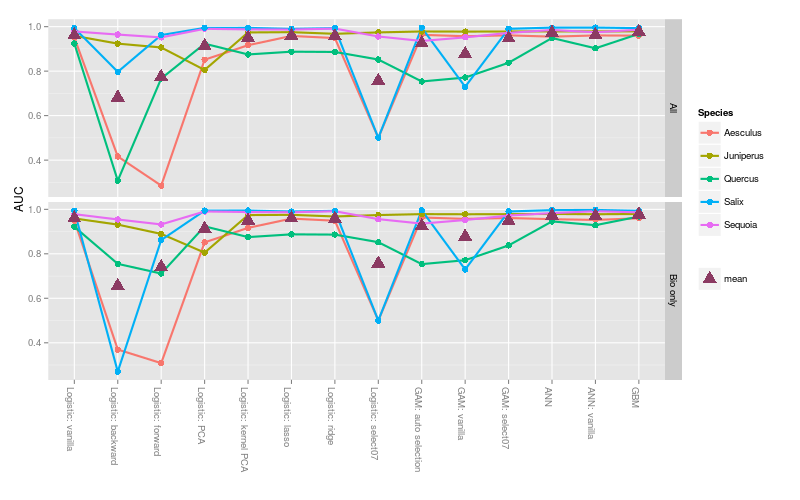
\includegraphics[scale=0.70]{Plots/AUCPAPlot.png}
}
\end{figure}

\section{Discussion}